\documentclass[bachelor, nocolorlinks, printoneside]{seuthesis} % 本科
\usepackage{tikz}

\usepackage{amsmath}
\usepackage{amssymb}
\usepackage{esint}
\usepackage{CJK,CJKnumb}
\usepackage{amsfonts} 
\usepackage{bm}
\usepackage{algorithm}
\usepackage{algorithmicx}
\usepackage{algpseudocode}
\usepackage{subfigure}


\floatname{algorithm}{算法}
\renewcommand{\algorithmicrequire}{\textbf{输入:}}
\renewcommand{\algorithmicensure}{\textbf{输出:}}
 % 这里是导言区
\categorynumber{000} % 分类采用《中国图书资料分类法》
\UDC{000}            %《国际十进分类法UDC》的类号
\secretlevel{公开}    %学位论文密级分为"公开"、"内部"、"秘密"和"机密"四种
\studentid{61519322}   %学号要完整,前面的零不能省略。

\title{基于惩罚力的流固耦合方法研究}{}{Penalty based Fluid-Structure Interaction}{}
\author{杨哲睿}{Zherui Yang}
\advisor{刘利刚}{教授}{Ligang Liu}{Prof.}
\coadvisor{唐慧}{副教授}{Hui Tang}{Lecturer} % 没有

% \degree{工学硕士} % 详细学位名称
\major[12em]{计算机科学与技术}
\defenddate{答辩日期}
\authorizedate{学位授予日期}
\department{吴健雄学院}{department name}
\duration{2019年9月—2023年6月}
\address{东南大学}
\thanks{TODO}
\newcommand{\argmin}[1]{\mathop{\arg\min}\limits_{#1}}
\newcommand{\argmax}[1]{\mathop{\arg\max}\limits_{#1}}



\date{\today}

\begin{document}

% Title Page.
% TODO: Title Page
\maketitle

% Abstract
\begin{abstract}{物理仿真,流固耦合,计算机图形学}
  TODO
\end{abstract}


\begin{englishabstract}{Physical Simulation, Fluid-Structure Interaction, Computer Graphics}
  TODO
\end{englishabstract}

% TOC:
\tableofcontents
\begin{Main}
  
% Main body.
\chapter{绪论}
\section{课题背景和意义}

基于物理的模拟是计算机动画、计算机辅助设计的基础。基于物理的模拟的本质是对于带有初边值条件的、大规模偏微分方程的求解。其中,偏微分方程,即控制方程,来源于牛顿第二定律与不同属性物体的本构方程结合。初值条件来源于用户设定的初始位置、速度等固定信息。边值条件主要来源于物理上物体之间的相互作用,以及用户在模拟过程中设置的交互。物理模拟中,动力学解算主要是指对于控制方程的解算,在不考虑边值条件的情况下,求解物体的的受力情况。边界条件解算主要是求解不同物体在交界面上的力学特征。

在图形学相关的物理模拟中,通常使用较为简单的本构模型,例如使用线性超弹性模型、不可压缩流体模型、弹簧质点模型来简化复杂的、真实的物理模型。因此,图形学的物理模拟中,动力学解算通常较为简单且易于实现。但由于场景、交互复杂,边值条件的解算成为在物理仿真中更复杂的部分。然而,相较于大规模科学计算软件的物理仿真,图形学应用中的用户交互更为丰富,边值条件的求解也更复杂,且图形应用具有强实时交互的要求,提升边值条件的解算效率,是物理仿真中的一大问题。

研究拥有不同材料控制方程物体之间的运动耦合方法,特别是流体-固体耦合方法是基于物理的模拟应用中的一个重要课题。流固耦合是指流体和固体之间相互作用的过程。在这个过程中,流体对固体施加压力,改变固体的形状和运动状态;同时,固体的形状和运动状态的变化也会影响流体的流动。基于惩罚函数法的流固耦合物理仿真,旨在通过流体、固体的控制方程对二者分别进行运动学建模,并利用惩罚函数对物体间相互作用进行统一建模,对复杂多物体场景的物理仿真提供了技术支撑。

研究流固耦合方法,主要目的在于优化现有计算机动画框架中的流体建模和求解算法的性能,提升计算机动画中流体的真实感,提升物理引擎仿真计算速度。而惩罚函数法是处理不同物体之间的约束的常见方法,其代码实现简单,在应用隐式时间积分器的时,拥有较高的数值稳定性。

传统的流固耦合方法常常基于上一时间步的固体速度和求解出的流体压强来计算下一时间步的物理量。尽管该方法可以将流固的计算分离,实现上较为简单,但也引入了较大的误差。例如,在重力场下的物体进入原本平衡的水面时,流体会晚于固体运动,从而发生流体到固体内部的穿透问题。基于惩罚函数法可以发现其中的穿透并将其转化为惩罚函数进行处理,能够有效消除穿透问题,并提供更为准确的流固耦合结果。

\section{本文研究内容}

本文主要提出了一个基于惩罚力实现流固运动耦合的算法。该算法采用物质点法实现流体模拟,有限元法和弹簧质点模型实现固体模拟。在耦合上,将物理上的碰撞视为约束,使用内点罚函数法模拟了流体粒子与固体的力相互作用。基于内点法的基本原理,本文应用了交替方向乘子法实现了计算加速。本文在多个场景下进行了测试,实验结果表明,该方法能够有效地解决流固之间的动力学耦合问题。

与此同时,本文还讨论了实验中使用的弹性体/布料/流体的运动学解算器(\ref{sec:dyn-solve}、\ref{sec:experiment-admm}节) 、二阶段碰撞检测的实现与测试(\ref{sec:collid-detect}节)。本文中采用的布料模拟算法、有限元算法和碰撞检测算法,相比先前的算法在相同条件下具有数倍的计算性能领先。

\section{论文各章节安排}

第\ref{chap:rel-works}章简要介绍了现有的流固运动学原理与求解方法、流固耦合的现有算法与惩罚函数法的应用。第\ref{chap:my-work}章详细描述了增量势能接触(IPC)及改进的ADMM-IPC流固耦合算法。第\ref{chap:experiment}章展示了ADMM-IPC算法的实现细节与测试结果。最后,第 \ref{chap:no-future} 章对于本文提出的方法进行了讨论与展望。

\chapter{相关工作}\label{chap:rel-works}

\section{动力学方程及其离散化}

物理仿真的核心是对于动量PDE的求解:
\begin{equation}
\mathbf F(\mathbf x, t) = M \ddot{\mathbf x}  
\end{equation}
根据物体属性的不同、数学离散化的不同,可以给出该方程的不同离散形式。

% Ref: https://innovationatwork.ieee.org/the-advantages-of-fem/
有限元方法(FEM)是一种用于数值求解工程和数学建模中微分方程的流行方法。它通常用于结构分析、传热、流体流动、质量传输和电磁势等领域。有限元方法有许多优点。例如,它允许更容易地对复杂的几何形状和不规则形状进行建模。有限元方法基于物体的拉格朗日网格表示实现。其将复杂的物体视为简单物体的组合,例如使用三角元、六面体元对于原物体进行剖分,通过计算大量的简单物体的物理量变化,来逼近整个复杂物体的物理量变化。

弹簧质点模型是一种抽象的物理系统,它假设模拟对象要么是质点,要么是弹簧,质点之间通过弹簧连接。经过这样的抽象,要模拟整个系统的物理运动,只需要模拟弹簧质点分别的运动和它们之间的关系即可。弹簧质点模型是对于布料建模的常用手段。

有限体积法(FVM)是一种以数值方法解偏微分方程的计算方式。在有限体积法中,将要描述的物理实体切分为网格单元来描述,并使用散度定理,将所有包含散度项的偏微分方程中的体积积分转换为表面积分。对于流体而言,给定模拟区域,有限体积法将区域进行固定的网格划分,在网格点上存储速度、密度物理量。每一时间步,都根据控制方程的欧拉形式进行解算和更新。

物质点法(MPM)是一种混合拉格朗日/欧拉的PDE求解方法,最近被引入计算机图形学领域。它使用控制方程的连续性描述,并利用用户可控的弹塑性本构模型。MPM允许使用规则的笛卡尔网格来自动的总碰撞和断裂处理。基于MPM原理提出的FLIP算法已经成为流体仿真的经典。

本节将简要介绍 FEM 变形体、弹簧-质点模型布料、MPM方法流体的力学、运动学求解基本原理和算法。本文所考察的物理现象都在三维空间中进行,并在不引起歧义的情况下,不区分各类张量本身与其在标准笛卡尔坐标系下的坐标符号。


\subsection{有限元模型的变形体解算}\label{sec:dyn-solve}

给定几何形体上的 $N$ 个采样点,$\mathbf x_{i}, i = 1\cdots N$,及其剖分得到的单元集合(以四面体为例)$\mathcal T = \{(i, j, k, l)\}$,通过计算采样点的运动,逼近整个几何形体的运动。

图形学中,常用三角元对物体进行剖分,并使用线性基函数对物理量进行插值逼近。运动学模拟求解的是形变函数
$$
\mathcal F: \Omega_0 \rightarrow \Omega_t
$$
其中$\Omega_0$表示初始状态下的物体,$\Omega_t$表示$t$时刻的物体,$\mathcal F$将 $\Omega_0$ 的一点一一地映射到$\Omega_t$上的一点。考虑$t = 0$其上的采样点$\mathbf x_i(0)$,$\mathbf x_i(t) = \mathcal F(\mathbf x_i(0))$。所谓线性基函数是指,对于某个四面体元中$(i, j, k, l)$的任一点 $\mathbf x(0)$,其$t=0$时刻的重心坐标为$(u, v, w)$,则近似其$t$时刻的位置为
$$
\mathbf x(t) = u \mathbf x_j(t) + (1 - u)\mathbf{x}_i(t) + 
 v \mathbf x_k(t) + (1 - v) \mathbf{x}_i(t)
 + w \mathbf x_l(t) + (1 - w) \mathbf{x}_i(t)
$$


\begin{figure}[h!]
  \centering
  \includegraphics[width=0.9\linewidth]{img/Screenshot 2023-04-19 at 10.23.09.png}
  \caption{有限元法空间离散化:将物体离散为四面体,在空间上存储四面体节点的位置与速度,在拓扑上存储节点的四面体连接关系。}
\end{figure}

为描述物体在局部的形变情况,定义物体形变梯度为:
\begin{equation}\label{def:def-grad}
  \mathbf F = \nabla_{\mathbf x} \mathcal F
\end{equation}
对于四面体元$(i, j, k, l)$,利用静止状态和当前状态的位置坐标$\mathbf x_i(0), \mathbf x_i(t)$,计算形变梯度为
\begin{equation}\label{eq:deformation-grad-compute}
\begin{aligned}
  \mathbf F =\mathbf X_{\mathrm{curr}}\mathbf X_{\mathbf{rest}}^{-1} =& [\mathbf x_j(t) - \mathbf x_i(t);\mathbf x_k(t) - \mathbf x_i(t); \mathbf x_l(t) - \mathbf x_i(t)] \\
  &\cdot [\mathbf x_j(0) - \mathbf x_i(0);\mathbf x_k(0) - \mathbf x_i(0); \mathbf x_l(0) - \mathbf x_i(0)]^{-1}
\end{aligned}
\end{equation}

根据线性有限元的基本假设,形变梯度在每一个四面体元$i$中为常量,记为$\mathbf F_i$。在空间中引入笛卡尔坐标系,$\mathbf x \in {\mathbb R}^3, \mathbf F_i \in \mathbb{R} ^{3\times 3}$。矩阵$\mathbf F_i$描述了该四面体元的形变情况。

当前,我们主要考虑超弹性模型。在形变中,超弹性模型保证了弹性能有如下性质:
\begin{enumerate}
  \item 旋转不变性:对于物体的旋转操作不改变弹性能量;
  \item 平移不变性:对于物体的平移操作不改变弹性能量;
\end{enumerate}
其弹性能量密度函数$\Psi$仅依赖于$\mathbf F$。若考虑矩阵 $\mathbf F$的 SVD 分解
\begin{equation}\label{eq:def-grad-svd}
  \mathbf F = U \Sigma V^T
\end{equation}
由于超弹性模型的平移不变性,$\Psi$仅由$\Sigma=\mathrm{diag}(\sigma_1, \sigma_2, \sigma_3)$决定。

常见的超弹性模型有 StVK模型、Neo-Hookean模型等。弹性能量密度函数的不同定义与材料参数 $\lambda, \mu$ 的设置,区分了不同材料的力学特性:
\begin{equation}\label{eq:stvk-phi}
  \Psi_{\mathrm{stvk}} = \frac{1}{2} \| \mathbf F' \mathbf F - \mathbf I\|_F^2 = \frac{1}{2} \|\mathbf E\|_F^2 
\end{equation}
\begin{equation}
  \label{eq:neohookean-phi}
  \Psi_{\mathrm{NeoHookean}} = \frac{\mu}{2} (\|\mathbf F\|_F^2 - 3)- \mu \log \det \mathbf F + \frac{\lambda}{2}\left(\log{\det \mathbf F}\right) ^2
\end{equation}

弹性能量密度函数对$\mathbf F$的微分$\mathbf P = \nabla_{\mathbf F} \Psi$给出了物体该位置的应力张量。

在线性有限元计算时,由于$\mathbf F$在内部为常数,四面体各顶点受力为:
\begin{equation}
  \mathbf f =V\cdot \nabla_{\mathbf x_i(t)} \Psi(\mathbf F_i)\label{eq:force-fem}
\end{equation}
其中$V$为该四面体体积。公式\ref{eq:force-fem}直接给出了有限元模拟中弹性力的计算方法。对于每一个采样点$i$,都有可能出现在多个四面体中,需要将相关的力进行求和,得到汇总后的弹性力。

\subsection{弹簧质点模型布料解算}

弹簧质点模型常用于布料的建模,建立的布料模型通常具有如下的网格结构
\begin{figure}[hbt]
\centering
  \includegraphics[width=0.4\linewidth]{img/Screenshot 2023-04-19 at 18.56.20.png}
  \caption{布料的弹簧质点模型:每一个顶点表示一个质点,在质点上记录速度与位置信息,每一条线表示一个弹簧,具有原长、劲度系数参数。}
\end{figure}

弹簧$(i, j)$的力学性质直接由胡克定律给出,弹簧对于质点 $j$ 的力为:
\begin{equation}
  \mathbf f = k(\| \mathbf x_i - \mathbf x_j\| - l_0) \frac{\mathbf x_i - \mathbf x_j}{\|\mathbf x_i - \mathbf x_j\|}
\end{equation}

与FEM类似,对于同一质点,需要计算与之相连的所有弹簧对其的作用力。

\subsection{隐式运动学解算}

宏观低速物体运动学方程由牛顿第二定律方程给出:
\begin{equation}
  \label{eq:newton2nd}
  \mathbf f_i = m_i \ddot{\mathbf x}_i
\end{equation}
其中,$\mathbf f_i$为物体 $i$ 的合外力,$m_i$为物体或采样点的质量。对于系统中有多个质点的情况,可以将方程改写为如下的矩阵形式:
\begin{equation}
  \label{eq:newton2nd-mat}
  {\mathbf f }= M{\mathbf x}
\end{equation}
其中:
$$
{\mathbf f} = \begin{bmatrix}
  \mathbf f_1\\
  \vdots\\
  \mathbf f_n
\end{bmatrix}\quad
\mathbf x =  \begin{bmatrix}
  \mathbf x_1\\
  \vdots\\
  \mathbf x_n
\end{bmatrix}\quad
M =\mathrm{diag}(m_1, \cdots, m_n)\otimes \mathbb I_3
$$

显式方法和隐式方法都是数值求解偏微分方程的方法。显式方法使用欧拉公式将微分方程转化为差分方程,然后使用差分方程进行数值求解。这种方法简单易懂,计算速度快,但是精度相对较低。一阶显式时间积分格式为:
\begin{equation}
  \begin{cases}
    \mathbf x^{n+1} = \mathbf x^{n} + h\mathbf v^{n} \\
    \mathbf v^{n+1} = \mathbf v^{n} + hM^{-1} \mathbf f^{n}
  \end{cases}
\end{equation}
其中,上标$n$表示时间步步数,$h$表示时间步步长。

尽管显式方法实现简单,但其稳定区域小,实现中容易出现数值爆炸的问题。计算机图形学的模拟中常用的是解决方案是隐式积分。隐式方法则使用隐式公式将微分方程转化为差分方程,然后使用迭代法进行数值求解。这种方法计算速度较慢,但是精度相对较高,且对于数值误差有较好的控制作用。
\begin{equation}
  \label{eq:1st-implicit}
  \begin{cases}
    \mathbf x^{n+1} = \mathbf x^{n} + h\mathbf v^{n} \\
    \mathbf v^{n+1} = \mathbf v^{n} + hM^{-1} \mathbf f^{n+1}
  \end{cases}
\end{equation}
将公式\ref{eq:1st-implicit}中的$\mathbf v^{n+1}$项消去
\begin{equation}
  \label{eq:impl-eqt}
  \mathbf x^{n+1} = \mathbf x^{n}+h\mathbf v^{n} + h^{2} M^{-1}\mathbf f^{n+1}
\end{equation}

在\ref{sec:dyn-solve}节讨论的、以及物理模拟中的绝大部分内力$\mathbf f_{int}$都是时间无关的,即$\mathbf f_{int}$ 是 $\mathbf x$ 的函数。同时系统外力$\mathbf f_{ext}$在单个时间步内为定值,故隐式积分\ref{eq:impl-eqt}可转化为关于$\mathbf x$的非线性方程组:
\begin{equation}
  \mathbf x^{n+1} = \mathbf x^{n}+h\mathbf v^{n} + h^{2} M^{-1}(\mathbf f_{int}(\mathbf x^{n+1}) + \mathbf f _{ext}^{n+1})
\end{equation}
在不考虑摩擦等能量耗散,系统内力都是保守力的情况下(存在势能函数$\Psi$,使得$\mathbf f = - \nabla_{\mathbf x} \Psi$),通过变分法将方程求解问题转化为能量最小化问题:% Ref:IPC 中的几个文章, Ref:https://zh.wikipedia.org/zh-hans/最小作用量原理#歐拉-拉格朗日最小作用量原理
\begin{equation}\label{eq:impl-opt-of}
  \mathbf x^{n+1} = \argmin{\mathbf x} E(\mathbf x) = \argmin{\mathbf x} I(\mathbf x) + \Psi(\mathbf x) = \argmin{\mathbf x} \frac{1}{2h^2} \| \mathbf x - \mathbf y\|_M^2 + \Psi(\mathbf x)
\end{equation}
其中的$I$描述了物体的惯性,$\mathbf y$表示了考虑系统外力和惯性的位置向量:
\begin{equation}
  \mathbf y = \mathbf x^{n} + h \mathbf v^{n} + h^2 M^{-1} \mathbf f_{ext}
\end{equation}
至此,隐式时间积分问题转化为优化问题,可采用各类基于梯度和Hessian矩阵的数值优化算法进行优化求解。通用的方法有带线搜索的牛顿迭代法等。

以弹簧质点模型为例,设系统中的所有弹簧集合为$\mathcal T = \{ (i, j) \}$,弹簧原长为$l_{0,(i,j)}$,则所有弹簧的总弹性势能为:
\begin{equation}
  \Psi_{\mathrm{MassSpring}} = \sum_{(i, j) \in \mathcal T} \frac{1}{2}(\| \mathbf x_i - \mathbf x_j\| - l_{0, (i, j)})^2
\end{equation}
代入式\ref{eq:impl-opt-of}中,可得
\begin{equation}\label{eq:mass-spring-opt-problem}
  \mathbf x^{n+1} = \argmin{\mathbf x} I(\mathbf x) + \sum_{(i, j) \in \mathcal T} \frac{1}{2}(\| \mathbf x_i - \mathbf x_j\| - l_{0, (i, j)})^2
\end{equation}
记$\mathbf x_{ij} = \mathbf x_i - \mathbf x_j$并对优化函数取某一质点位置的偏导可得:
\begin{equation}\label{eq:mass-spring-gradient}
  \begin{aligned}
    \nabla_{\mathbf x_i} E(\mathbf x) &= \frac{1}{h^2}M (\mathbf x_i - \mathbf y_i) +\sum_{(i, j) \in \mathcal T} \frac{\partial \Psi}{\partial \|\mathbf x_{ij} \|} \frac{\partial \|\mathbf x_{ij} \|}{\partial \mathbf x_i} \\
    &=\frac{1}{h^2} M (\mathbf x_i - \mathbf y_i) + \sum_{(i, j) \in \mathcal T} (\| \mathbf x_{ij} \| - l_{0, (i, j)})\frac{\mathbf x_{ij} }{\|\mathbf x_{ij} \|}
  \end{aligned}
\end{equation}

结合上式给出的梯度,采用最速下降法与线搜索进行实现:
\begin{algorithm}
  \caption{最速下降法解弹簧质点系统}
  \begin{algorithmic}[1]
    \Require 弹簧集合 $\mathcal T$,当前位置$\mathbf x^{n}$和惯性项位置$\mathbf y$,最大迭代次数$N$,误差限$\varepsilon_0$
    \Ensure 积分结果 $\mathbf x^{n+1}$
    \State $\mathbf x\leftarrow \mathbf y$, $i \leftarrow 1$
    \State $\mathbf d \leftarrow - \nabla_{\mathbf x}E(\mathbf x)$, $\varepsilon \leftarrow \|\mathbf d\|$
    \While{$\varepsilon > \varepsilon_0$ and $i < N$}
      \State $\alpha\leftarrow 1$
      \State $\mathbf x'\leftarrow \mathbf x + \mathbf d$
      \While{$E(\mathbf x') - E(\mathbf x) > - 0.7 \alpha \| d \|$}
        \State $\alpha \leftarrow 0.7 \alpha$
        \State $\mathbf x' \leftarrow \mathbf x + \mathbf d$
      \EndWhile
      \State $\mathbf x \leftarrow \mathbf x'$
      \State $\mathbf d \leftarrow - \nabla_{\mathbf x}E(\mathbf x)$, $\varepsilon \leftarrow \|\mathbf d\|$
    \EndWhile
    \State \Return $\mathbf x$
  \end{algorithmic}
\end{algorithm}


\subsection{交替方向乘子法(ADMM)}\label{sec:admm}

% Ref: Fast Mass Spring, PD.
2014年,Liu 等人提出了投影动力学方法(Projective Dynamics,PD),用于弹簧质点模型的加速求解。其核心思想是使用Local/Global迭代求解弹簧质点模型的隐式积分方程。其使用了松弛变量 $\mathbf z_{ij}$ 作为弹簧中间变量,将原优化问题\ref{eq:mass-spring-opt-problem}转化为如下的交替迭代形式:
\begin{equation}\label{eq:mass-spring-pd}
  \begin{aligned}
    \text{Local Step}: & \quad\mathbf z_{ij} \argmin{\mathbf z_{ij}} = \|\mathbf x_i-\mathbf x_j - z_{ij}\| = \frac{\mathbf x_i-\mathbf x_j}{\|\mathbf x_i-\mathbf x_j\|} l_{0, (i, j)}\\
    \text{Global Step}: & \quad \mathbf x = \argmin{\mathbf x} I(\mathbf x) +\sum_{(i, j) \in \mathcal T} \frac{1}{2} \| \mathbf x_i-\mathbf x_j -\mathbf z_{ij}\|
  \end{aligned}
\end{equation}
其中 Local Step 对于每一个弹簧是相互独立的,可以在多处理器上并行处理,Global Step 是无约束的二次优化问题,可用 Cholesky 分解预处理稀疏的Hessian矩阵加速,极大地加速求解速度。同时,若该迭代格式收敛,则收敛到原问题的最优解。同样的原理也适用于基于Shape Matching的软体仿真以及部分的有限元仿真方法。

% ADMM ⊇ Projective Dynamics: Fast Simulation of Hyperelastic Models with Dynamic Constraints
% Ref: Distributed Optimization and Statistical Learning via the Alternating Direction Method of Multipliers (Boyd, Parikh, Chu, Peleato, Eckstein)
2017年,Overby 等人提出,PD方法仅仅是交替方向乘子法的一个特例。交替方向乘子法(Alternating Direction Method of Multipliers,ADMM)是一种求解带有等式约束的优化问题的算法。它通常用于解决存在两个优化变量的只含等式约束的优化类问题。该算法将原问题分解为两个子问题,分别对每个子问题进行求解,然后通过交替更新乘子来保证收敛。ADMM算法的主要优点是可以处理大规模问题,并且可以在分布式计算环境中使用。

对于等式约束的优化问题\ref{eq:eql-opt-prob}:
\begin{equation}\label{eq:eql-opt-prob}
\begin{aligned}
  \argmin{\mathbf x,\mathbf z}&\quad F(\mathbf x)+G(\mathbf z)\\
  \mathrm{s.t.}&\quad \mathbf A\mathbf x +\mathbf B\mathbf z = \mathbf d
\end{aligned}  
\end{equation}
ADMM 方法将等式约束转化为拉格朗日乘子形式,给出如下目标函数:
\begin{equation}
  L_{\rho}(\mathbf x,\mathbf z,\mathbf u)= F(\mathbf x)+G(\mathbf z)+\mathbf u^{T}(\mathbf A\mathbf x+\mathbf B\mathbf z-\mathbf d)+\rho/2 \|\mathbf A\mathbf x+\mathbf B\mathbf z-\mathbf d\|_{\hat H}^{2}
\end{equation}
其中,$\| \cdot \|_{\hat H}$ 表示$\hat H$范数。给定迭代初值$\mathbf x^{(0)}$ 以及 $\mathbf u^{(0)} = 0$,ADMM迭代算法如下:
\begin{equation}\label{eq:admm-algorithm}
  \begin{aligned}
    \mathbf z^{(k)} &= \arg\min_{x} L_{\rho}(\mathbf x^{(k)},\mathbf  z, u^{(k-1)})\\
    \mathbf u^{(k)} &= \mathbf u^{(k-1)} + \rho(\mathbf{Dx}-\mathbf{z})\\
    \mathbf x^{(k+1)} &= \arg\min_{x} L_{\rho}(\mathbf x, \mathbf z^{(k)}, \mathbf u^{(k)})
  \end{aligned}
\end{equation}

将ADMM与PD公式\ref{eq:mass-spring-pd}对照可知,投影动力学方法的实质是具有如下参数的ADMM方法:
\begin{equation}
  \mathbf u \equiv 0,\quad \rho = \begin{cases}
    \infty & \text{in Local Step}\\
    1 & \text{in Global Step}\\
  \end{cases}, \quad\hat H = \mathbb I_3
\end{equation}
在后续的工作中指出$\rho$的合理选取影响了ADMM的收敛速度,对于弹簧质点模型而言,$\rho = 1$ 是一个较合理的选择。对于有限元物体,考察四面体$(i,j,k,l)$,Overby 等人选取$\mathrm{vec}(\mathbf X)$作为ADMM算法中的$\mathbf z_{ijkl}$进行优化迭代,并选取$\hat H=\mathbb I_{9}, \rho =  0.7(\lambda + 2\mu)$来实现松弛。

对于本论文实现的布料、有限元求解器,为提高系统并行性能、减少重复计算,采用了(Jacobi迭代的)Consensus ADMM方法,并选择了$\mathbf F$ 作为松弛变量,更多实现细节请见\ref{sec:experiment-admm}节。

\subsection{有限体积法与物质点法流体动力学解算}\label{sec:fvm-mpm-fluid}

图形学中的流体力学解算使用完全不可压缩的纳维-斯托克斯方程(N-S方程):
\begin{equation}\label{eq:naiver-stokes-origin}
\begin{aligned}
\frac{\partial \mathbf u}{ \partial t} + \mathbf u \cdot \nabla \mathbf u + \frac 1 {\rho} \nabla p
&= \mathbf g + \nu\nabla ^2 \mathbf u\\
\nabla \cdot \mathbf u& = 0
\end{aligned}
\end{equation}
其中,$\mathbf u$表示流体的速度场。在数值求解时,常使用算符分裂法将PDE拆分为非压强部分和压强部分。这种方法可以大大简化计算,提高计算效率:% Ref: Fluid Simulation for Computer Graphics
\begin{equation}
  \begin{aligned}
    \frac{D q}{D t} & = 0 &(\text{Advection})\\
    \frac{\partial \mathbf u}{\partial t} & = \mathbf{f}_{\mathrm{ext}}\\
    \frac{\partial \mathbf u}{\partial t} + \frac{1}{\rho} \nabla p& = 0 &(\text{Pressure Projection})\\
    \text{such that }\nabla \cdot \mathbf u &= 0
  \end{aligned}
\end{equation}
通过分别求解Advection步和Pressure Projection步实现完整时间步的求解。

Pressure Projection,即流体的压强计算,由流体的不可压缩性,或速度场无散条件给出连续方程。其实质是一个关于空间压强场的泊松方程:
\begin{equation}
  \label{eq:fluid-poisson}
  \nabla \cdot \mathbf u^{n+1} = \nabla \cdot (\mathbf u^{A} - \Delta t \frac{1}{\rho} \nabla p) = 0 \implies \Delta t \frac{1}{\rho} \nabla \cdot \nabla p = \nabla \cdot \mathbf u^{A}
\end{equation}
其中$\mathbf u^{A}$为经过Advection步得到的含散度的速度场。

一般而言,FVM方法将整个模拟区域按 $\Delta x$ 划分为均匀网格,并存储网格点处的物理量信息,例如速度场$\mathbf u_{i,j,k}$。其相较于有限元方法而言,由于划分均匀且不随时间变化,空间微分算符 $\nabla$ 具有更简单的离散形式,例如二阶精度的中心差分:
\begin{equation}
  \nabla\cdot \mathbf u \approx 
  \frac{1}{2\Delta x}\left(\mathbf u_{i+1,j,k}-\mathbf u_{i-1,j,k} +
    \mathbf u_{i,j+1,k}-\mathbf u_{i,j-1,k}+
  \mathbf u_{i,j,k+1}-\mathbf u_{i,j,k-1}\right)
\end{equation}
利用各个算符的离散微分形式,可以得到方程\ref{eq:fluid-poisson}的离散形式。由于离散拉普拉斯算子的正定性,对该矩阵方程,常用结合了多重网格和矩阵预分解的共轭梯度法(Multi-Grid Preconditioned Conjugated Gradient, MGPCG)进行求解。

FVM的问题之一是,对于速度和密度的时间算符求解较为复杂,导致Advection步有较大的计算开销,并带来较大的数值耗散现象。MPM法解决了这一问题。MPM通过在采样点上进行运动学解算,在均匀网格上进行动力学解算。时间求解时,其利用FVM的动力学解算的速度场,执行采样点位置坐标在给定速度场上的时间ODE求解。动力学求解时,从采样点上插值空间中格点的动量和密度。通用的MPM算法流程如图\ref{fig:mpm-overview}所示:
\begin{figure}[hbt]
  \centering
  \includegraphics[width=0.98\linewidth]{img/Screenshot 2023-04-19 at 19.55.25.png}
  \caption{MPM 算法流程:上半部分为拉格朗日粒子,下半部分为欧拉网格,通过插值操作进行相互传递。}\label{fig:mpm-overview}
  % Ref:CJFF
\end{figure}

MPM方法推导过程中,称采样点为拉格朗日粒子,背景网格为欧拉网格。在拉格朗日粒子和欧拉网格之间的信息传递通过守恒方程插值实现。给定具有局部支撑集的插值基函数,$W(\mathbf x)$,从粒子到位置为$\mathbf x_{i,j,k}$网格点的插值由如下公式给出,反之亦然:
\begin{equation}\label{eq:mpm-transf}
\begin{aligned}
  &\text{质量守恒}\quad & m_{i,j,k} &= \sum_{p} m_{p} W(\mathbf x_{i,j,k}- \mathbf x_p)\\
  &\text{动量守恒}\quad & m_{i,j,k}\mathbf u_{i,j,k} &= \sum_{p} m_{p} \mathbf v_{p}W(\mathbf x_{i,j,k}- \mathbf x_p)
\end{aligned}
\end{equation}
通常,$W(\mathbf x)$选为三次B-样条函数:
\begin{equation}
  W(\mathbf x) = \begin{cases}
    \frac{1}{2}\| \mathbf x\| ^3 - \| \mathbf x\|^2 +\frac{2}{3} & 0 \le \| \mathbf x\| < 1\\
    \frac{1}{6}\left(2 -\| x \| \right)^3 & 1 \le \| \mathbf x\| < 2\\
    0 & 2 \le \| \mathbf x\|\\
  \end{cases}
\end{equation}

一个精简的MPM时间积分算法如下。本设计中实现的流体力学解算器采用了Affine PIC格式插值。Affine PIC方法相较于公式 \ref{eq:mpm-transf} 对于角动量的保持更加高效。对于无散条件,采用显式方法来控制密度变化,获取更高的计算速度。
\begin{algorithm}[H]
  \caption{MPM 时间积分}
  \begin{algorithmic}[1]
    \label{algo:mpm-time-integration}
    \Require 流体粒子系统位置$\mathbf x^n$,速度$\mathbf v^n$,时间步长$h$
    \Ensure 积分结果 $\mathbf x^{n+1}, \mathbf v^{n+1}$
    \State $\mathbf x ^{n+1} \leftarrow \mathbf x^{n} + h \mathbf v^{n}$
    \State 对 $\mathbf x$ 用公式 \ref{eq:mpm-transf} 计算网格数据 $\mathbf u^{n}$
    \State 对 $\mathbf u^{n}$ 求解无散速度场 $\mathbf u^{n+1}$
    \State 使用公式 \ref{eq:mpm-transf} 恢复粒子速度 $\mathbf v^{n+1}$
    \State \Return $\mathbf x^{n+1}, \mathbf v^{n+1}$
  \end{algorithmic}
\end{algorithm}

\section{流固耦合}

流固耦合是指流体和固体之间的相互作用。因为流体对固体的运动产生反作用力,而固体对流体的运动也产生反作用力,流体和固体之间的相互作用是双向的。这种相互作用在许多工程领域中都很重要,例如航空航天、汽车工程、建筑工程等。在大规模的科学计算应用中,流固耦合通常会采用有限元或边界元法,结合贴体网格或浸没边界法,对流固边界建模并解算。但在图形学应用中,通常采用一些近似化方法对于流固耦合作用进行求解。

本节将简要介绍图形学流固耦合和碰撞处理常用的方法。其中,固体指代前文中的网格化物体,即布料、可变形体,流体则特指使用MPM方法进行模拟,具有粒子表示。

尽管在工程领域,材料的温度、状态等都会对于作用力产生影响,但在图形学中,常常忽略其他物理量,而只考虑流体与固体之间不发生穿透的简单情形。从数学上描述,给定固体上一点$\mathbf x$及在该处的表面外法向 $\mathbf n$和速度 $\mathbf v$,若流体在该处速度为$\mathbf u$,那么在该处应满足:
\begin{equation}\label{eq:coupling-velocity}
  0 \le -\langle \mathbf v - \mathbf u, \mathbf n \rangle \perp -(\mathbf f_{f\rightarrow s} \cdot \mathbf n) \ge 0
\end{equation}
即在法向上,固体速度分量大小不大于流体速度分量大小。若不然,流体会穿透固体表面进入其内部。

公式 \ref{eq:coupling-velocity} 给出了运动学方程 \ref{eq:newton2nd} 和 \ref{eq:naiver-stokes-origin} 的边界条件。对于该边界条件,从固体是否能影响流体的运动、固体是否是刚体两方面区分,有如下四种处理方法:
\begin{enumerate}
  \item 单向耦合:适合固体小颗粒与流体的耦合,固体的运动完全由每一时刻的流体速度场决定,固体无法改变流体的运动;
  \item 弱耦合:在一个时间步内先后解算流体与固体,将流体解算时固定当前固体速度为边界条件,固体解算时固定当前流体压强场计算受力,需要较小的时间步长;
  \item 强耦合:在一个时间步同时进行流体与固体求解,来保证其不产生分离或穿透现象,但实现复杂且计算效率低下;
  \item 浸没边界法:类似于物质点法,通过建立浸没边界,在背景网格和网格物体之间建立物理量联系,是CFD中常见的方法,需要较大的计算和存储开销。
\end{enumerate}

上述四种方法是使用FVM网格下流体模拟进行流固耦合的常用方法,同样也适用于MPM流体与固体的耦合。本节将简要描述单向耦合、弱耦合、以及浸没边界法,强耦合算法复杂度较高,在此不再赘述。

\subsection{单向耦合}

单向耦合基于固体无法影响流体运动的假设,并且根据固体的惯性大小来决定使用何种模型:对于惯性较小的固体,可以直接设置固体的速度为该处的流体速度;对于以速度$\mathbf v$运动的,有一定惯性的物体,可以设置 $\mathbf f = k (\mathbf u - \mathbf v)$ 作为流体对其施加的外力,来进行流固耦合。

\subsection{弱耦合}

弱耦合是图形学中最常用的流固耦合方法。其核心思想是对于流体的求解,假设固体的运动是其边界条件,固体求解中流体压强不变,且贡献一份外力。其基本思路如下:
\begin{enumerate}
  \item 更新流体位置:流体 Advection;
  \item 求解所有流体的非压强受力;
  \item 当前固体的速度作为边界条件,求解流体压强;
  \item 流体压强作为施加在固体上的外力,考虑碰撞等因素,求解固体
\end{enumerate}

其中第 1、2、3 步都是已经在前文介绍的算法(见\ref{sec:dyn-solve}、\ref{sec:fvm-mpm-fluid}节),对于压强求解,通常考察压强场在固体边界的面积分:
\begin{equation}
  \label{eq:pressure-field-integration}
  \mathbf f_{f\rightarrow s} = \oiint_{\partial \Omega} \hat{\mathbf n} dS
\end{equation}
其中,$\hat{\mathbf n} = p \mathbf n$,$p$为流体压强,$\mathbf n$为单位法向量。对于该面积分通常采用散度定理,将复杂的对固体表面的曲面积分,转化为简单的对FVM网格边界的积分:
\begin{equation}
  0 = \oiint_{\partial \Omega_i} \hat{\mathbf n} dS = \oiint_{\partial \Omega_{if}} \hat{\mathbf n} dS + \oiint_{\partial \Omega_{is}} \hat{\mathbf n} dS
\end{equation}
其中$\partial \Omega_{if}$与$\partial \Omega_{is}$如图\ref{fig:fluid-divergence-theo}所示。

\begin{figure}[hbt]
  \centering
  \includegraphics[width=0.9\linewidth]{img/diagram-20230501.png}
  \caption{散度定理}\label{fig:fluid-divergence-theo}
\end{figure}

弱耦合的一大问题是,由于流体与固体分开求解,即对于时间步 $n\rightarrow n+1$,第 $n$ 步的流体速度场$\mathbf u^n$、压强场$p^n$和固体速度$\mathbf v^{n}$:
\begin{enumerate}
  \item 基于$\mathbf v^n$计算流体压强$p^{n+1}$;
  \item 基于$\mathbf p^{n+1}$计算固体速度$\mathbf v^{n+1}$;
\end{enumerate}

因此,流、固之间在压强、速度变化较大时将产生较大的误差。例如,考虑一个即将落入水中且速度较快的的刚体球,在当前时间步的流体求解并不会考虑刚体球的边界条件,尽管固体速度求解时可能考虑压强影响,但在下一时间步,仍然会出现一定程度上的流体流入固体内部的错误。因此,弱耦合方法通常需要较小的时间步长,来减少由于不同时间步计算而产生的错误。

\subsection{浸没边界法}

浸没边界法是在计算流体力学中的常用方法。其总体思想类似于物质点法:
\begin{enumerate}
  \item 联合浸没边界,计算固体受力;
  \item 将浸没边界上的力传递到流体场上,作为外力求解;
  \item 求解不可压缩NS方程;
  \item 速度场传递到浸没边界上,更新浸没边界位置。
\end{enumerate}
浸没边界法是近年来CFD领域的研究重点,尽管算法简单,但时间、空间复杂度高,不适合于图形学应用,本文也不做过多描述。

\section{碰撞处理与惩罚函数法}\label{sec:collision}

2023年,Xie 等人指出,对于粒子描述下的流体,也可使用碰撞处理的方式来简化流固耦合操作。即将流体视为粒子,在网格物体与粒子之间直接应用各类碰撞处理算法,以解决原先的流固耦合问题。

碰撞处理是指在模拟物体运动时,当两个物体相撞时,如何计算它们的反弹方向和速度。这个过程通常包括检测碰撞、计算碰撞后的速度和方向、以及应用这些结果来更新物体的位置和速度。对于MPM流体而言,其粒子表示可以与其他网格化物体进行碰撞处理,以粒子与网格完全无弹性碰撞,来近似模拟流体与其他网格化物体的相互作用。碰撞处理可以分为两阶段:碰撞检测、碰撞响应。本节主要关注碰撞响应,碰撞检测算法设计与实现见\ref{sec:collid-detect}节。% TODO

几何上看,碰撞是指对于任意两个单纯复形,存在其中的两个不同单纯形之间的距离为$0$。将其中所有0-单纯形的位置视为自变量,距离为$0$实际描述了一个高维空间中的流形 $d(\mathbf x) = 0$。

考虑一维空间$\mathbb R$中的两个小球,其位置坐标分别为$x, y$,时间积分中的位置变量为$\mathbf x= (x, y)\in \mathbb R^{2}$。则两个小球碰撞是指 $d(\mathbf x) = x-y = 0$,如图\ref{fig:xy0}所示。

\begin{figure}[hbt]
  \centering
  

\tikzset{every picture/.style={line width=0.75pt}} %set default line width to 0.75pt        

\begin{tikzpicture}[x=0.75pt,y=0.75pt,yscale=-1,xscale=1]
%uncomment if require: \path (0,300); %set diagram left start at 0, and has height of 300

%Straight Lines [id:da29679656074971084] 
\draw    (221,232) -- (432,232) -- (438,232) ;
\draw [shift={(440,232)}, rotate = 180] [color={rgb, 255:red, 0; green, 0; blue, 0 }  ][line width=0.75]    (10.93,-3.29) .. controls (6.95,-1.4) and (3.31,-0.3) .. (0,0) .. controls (3.31,0.3) and (6.95,1.4) .. (10.93,3.29)   ;
%Straight Lines [id:da8887887549358049] 
\draw    (257,253) -- (257,91) ;
\draw [shift={(257,89)}, rotate = 90] [color={rgb, 255:red, 0; green, 0; blue, 0 }  ][line width=0.75]    (10.93,-3.29) .. controls (6.95,-1.4) and (3.31,-0.3) .. (0,0) .. controls (3.31,0.3) and (6.95,1.4) .. (10.93,3.29)   ;
%Straight Lines [id:da36164820457619884] 
\draw [color={rgb, 255:red, 208; green, 2; blue, 27 }  ,draw opacity=1 ]   (239,250) -- (384,106) ;
\draw   (301.04,149.39) -- (308.96,149.39)(305,145.43) -- (305,153.36) ;
\draw   (360.04,166.06) -- (367.96,166.06)(364,162.1) -- (364,170.02) ;
%Straight Lines [id:da4546673743664529] 
\draw [color={rgb, 255:red, 155; green, 155; blue, 155 }  ,draw opacity=1 ]   (305,150) -- (362.4,165.16) ;
\draw [shift={(364.33,165.67)}, rotate = 194.79] [color={rgb, 255:red, 155; green, 155; blue, 155 }  ,draw opacity=1 ][line width=0.75]    (10.93,-3.29) .. controls (6.95,-1.4) and (3.31,-0.3) .. (0,0) .. controls (3.31,0.3) and (6.95,1.4) .. (10.93,3.29)   ;

% Text Node
\draw (334,82.4) node [anchor=north west][inner sep=0.75pt]    {$x-y=0$};
% Text Node
\draw (287.33,119.4) node [anchor=north west][inner sep=0.75pt]    {$\mathbf{x}^{( k)}$};
% Text Node
\draw (369,164.4) node [anchor=north west][inner sep=0.75pt]    {$\mathbf{x}^{( k+1)}$};
% Text Node
\draw (450,215.4) node [anchor=north west][inner sep=0.75pt]    {$x$};
% Text Node
\draw (264,69.4) node [anchor=north west][inner sep=0.75pt]    {$y$};


\end{tikzpicture}

  \caption{距离为0约束}\label{fig:xy0}
\end{figure}

假定当前时间步的位置更新为$\mathbf x^{n} \rightarrow \mathbf x^{n+1}$,由隐式时间积分公式可知,我们认为在时间当前时间步内,所有的单纯形按照匀速直线运动,如下图所示。由于其中穿越了线性流形 $x-y = 0$,即存在时刻 $t \in [0, 1]$,使得$d(t \mathbf x_{n+1} + (1 - t) \mathbf x_{n}) = 0$ ,因此在这一时间步中发生了碰撞,需要进行正确的碰撞处理。


需要指出的是,碰撞处理的实质是避免让几何物体在任意时间发生相交,即距离为 $0$。因此,可以认为在时间积分的过程中存在一不等式约束,许多算法被提出以适应该约束。

%对于三位空间中的网格物体,仅需要考虑如下几类的单纯形之间的碰撞,即可实现几何形体之间的碰撞处理:
%\begin{enumerate}
%  \item 点-三角碰撞
%  \item 边-边碰撞
%\end{enumerate}
%对于维度更低的情况,例如点-边,点-点等碰撞将被纳入上述两类碰撞进行类似的检测和处理。
%Ref:Fast continuous collision detection using deforming nonpenetration filters Tangming.

惩罚函数法是用于碰撞响应的常用算法。其在计算机游戏、动画应用中都有较为广泛的应用。对于空间中的两个几何物体,惩罚函数法试图通过使用类似弹簧的恢复力来惩罚约束违规来避免碰撞的发生,从而实现碰撞处理。例如,考虑\ref{fig:penalty-force-illust}中所示的场景,其中连接了两个刚体的末端。作为惩罚方法的简单说明,我们添加一个原长为$0$的弹簧,用于连接刚体的两端,如下图所示。
\begin{figure}[hbt]
  \centering
  \includegraphics[width=0.5\linewidth]{img/Screenshot 2023-04-23 at 10.32.55.png}
  \caption{惩罚函数法处理碰撞:对于刚体1、2在碰撞点处建立弹簧,用弹簧的力来模拟碰撞的力,从而保证动量守恒。}\label{fig:penalty-force-illust}
\end{figure}

在时间积分时,计算该弹簧的受力,以避免两刚体的碰撞。惩罚函数法也可以不采用弹簧模型,而使用非线性的能量模型来避免需要人为设置的弹簧劲度系数参数。

惩罚函数法使用简单,但其确实存在缺点。例如,对于弹簧劲度系数$k$的设置,过高的的设置会将给系统引入额外的能量,过低的设置则不足以避免碰撞。而且,由于弹簧振动的性质,对于物体之间静止的场景难以用惩罚函数法实现。尽管如此,惩罚函数法仍然是用于处理约束、碰撞的一大类方法。

在数学上,惩罚函数法是在优化问题中处理约束的常用方法。惩罚方法用一系列无约束问题代替约束优化问题,这些问题的解理想地收敛于原始约束问题的解。无约束问题是通过在惩罚约束违规的目标函数中添加一项(称为惩罚项)而形成的。惩罚项在违反约束时较大,在满足约束时较小。惩罚方法依赖于迭代法求解,它从对解的初始猜测开始,然后反复求解一系列无约束问题,惩罚参数不断增加,直到收敛。%Ref Wikipedia

在图形学的碰撞处理中,由于一般的惩罚函数法在极端情况下不能保证没有相交情况,因此2020年 Li 等人提出了基于内点法的增量势能方法(Incremental Potential Contact, IPC)。内点法(也称为障碍函数法或IPM)是解决线性和非线性凸优化问题的一类算法,是惩罚函数法中的一类方法。内点法是一种迭代方法,它从对解的初始猜测开始,然后以越来越高的精度重复求解一系列线性或非线性规划问题,直到收敛。 % Ref: Wikipedia,IPC

增量势能接触(IPC)是一种用于变分求解隐式时间步长新模型和算法。它用于模拟接触变形固体的复杂相互作用。IPC 旨在对真实世界的接触弹性进行有效的时间步长精确和一致的仿真。IPC算法在原先隐式时间积分公式\ref{eq:impl-opt-of}的基础上,加入了距离非零的惩罚函数项 $B(\mathbf x)$
\begin{equation}\label{eq:barrier-func}
  B(\mathbf x) = \sum_{i \in \mathcal C} B(d_i(\mathbf x)), \quad B(d)= \begin{cases}
-(d - \hat d) ^ {2} \log \left(\frac{d}{\hat d}\right) & 0 < d < \hat d\\
0 & \mathrm{otherwise}
\end{cases}
\end{equation}
其中,$\mathcal C$ 表示所有可能的碰撞对,从而优化问题转化为一无约束的优化问题:
\begin{equation}\label{eq:ipc-opt-problem}
  \argmin{\mathbf{x}} E(\mathbf{x}) + B(\mathbf{x})
\end{equation}

在该框架下,碰撞处理转化为使用内点法迭代规避所有可能发生的碰撞,并在将要发生碰撞时,施加足够大的惩罚力。内点法要求每一次迭代更新 $\mathbf{x}^{(k)} \rightarrow \mathbf{x}^{(k+1)}$ 都满足
\begin{equation}
  \forall t \in [0, 1], E((1-t)\mathbf{x}^{(k)} + t \mathbf{x}^{(k+1))} + B((1-t)\mathbf{x}^{(k)} + t \mathbf{x}^{(k+1)}) < \infty
\end{equation}

\begin{algorithm}
  \caption{简化的IPC算法}\label{alg:ipc-sim}
  \begin{algorithmic}[1]
    \Require 当前位置$\mathbf x^{n}$
    \Ensure 积分结果 $\mathbf x^{n+1}$
    \State $\mathbf x^{(0)} \leftarrow \mathbf x^{n}$, $k \leftarrow 0$
    \State $\mathcal C \leftarrow \emptyset$
    \While{$\varepsilon > \varepsilon_0$ and $k < N$}
      \State $\mathbf d \leftarrow - H^{-1}\nabla_{\mathbf x}(E(\mathbf x) + B(\mathbf x))$
      \State 对 $\mathbf d$ 执行线搜索,确定系数$\alpha$
      \State $\mathbf x'\leftarrow \mathbf x + \alpha \mathbf d$
      \State 检查$\mathbf x^{(k)} \rightarrow x'$碰撞情况,最小碰撞时间为 $ 0 < \alpha' \le 1$,更新 $\mathcal C$
      \State $\mathbf x^{(k+1)} \leftarrow \mathbf x^{(k)} + \alpha' \mathbf d$
      \State $k\leftarrow k + 1$
    \EndWhile
    \State \Return $\mathbf x^{(k)}$
  \end{algorithmic}
\end{algorithm}


一个简单的IPC算法如\ref{alg:ipc-sim}所示。与原先论文的算法相比,该算法提炼了IPC的核心思想,即内点法:算法\ref{alg:ipc-sim}的第7、8步保证了每一次位置更新前都检查其更新轨迹不发生相交,从而处理了所有可能的碰撞。其中,算法的第4步中使用了优化函数的Hessian矩阵$H$获取更好的迭代方向,第5步使用线搜索,计算了一个可以使得目标函数充分下降的迭代步长。由于线搜索后执行了碰撞检测,并且该方向是一个下降方向,步长保证无碰撞发生,因此IPC确保了时间积分能够正确收敛到能量函数最小的位置,并且该时间步不发生穿透。

该算法的缺点在于,即使 $E$ 具有一个固定的 Hessian 矩阵,例如弹簧质点模型,由于 $B$ 的Hessian阵在每一个时间步都有可能发生变化,其也无法应用稀疏 Cholesky 分解等预计算加速方法进行快速矩阵计算。这对于复杂场景、复杂对象的解算是十分不利。

总而言之,对于碰撞处理问题,惩罚函数法是一类常用的解决方案。近年来,由于IPC算法的提出,基于内点法的碰撞处理又成为了研究焦点。对于流固耦合算法而言,可以转化为流体粒子与固体之间的完全非弹性碰撞,应用相关算法得以解决。本文的主要工作将从该重要的观察出发,进行基于惩罚函数法实现的流固耦合算法研究。


\chapter{ADMM-IPC}\label{chap:my-work}

\section{基于惩罚力的流固耦合}

流固耦合作用力的公式\ref{eq:coupling-velocity}给出了流固耦合的基本力学原理。对于该约束,若采用拉格朗日视角的流体描述,即可转化为流体粒子无法穿透任何固体表面的约束。我们考虑用该约束来实现流体粒子与固体的相互耦合。由于固体常用三角网格来表示,因此本章主要考虑的碰撞即为流体与三角网格的耦合。对于一个三角面与流体粒子,其碰撞如图\ref{fig:coupling-example}所示。

\begin{figure}\centering
\tikzset{every picture/.style={line width=0.75pt}} %set default line width to 0.75pt        
\begin{tikzpicture}[x=0.75pt,y=0.75pt,yscale=-1,xscale=1]
%uncomment if require: \path (0,300); %set diagram left start at 0, and has height of 300

%Shape: Circle [id:dp6935007166126634] 
\draw  [fill={rgb, 255:red, 175; green, 86; blue, 86 }  ,fill opacity=1 ] (298,81.5) .. controls (298,77.91) and (300.91,75) .. (304.5,75) .. controls (308.09,75) and (311,77.91) .. (311,81.5) .. controls (311,85.09) and (308.09,88) .. (304.5,88) .. controls (300.91,88) and (298,85.09) .. (298,81.5) -- cycle ;
%Shape: Triangle [id:dp09215856226306518] 
\draw  [fill={rgb, 255:red, 74; green, 144; blue, 226 }  ,fill opacity=0.59 ] (446.43,80.57) -- (389.12,228.06) -- (228.44,134.69) -- cycle ;
%Straight Lines [id:da9852007763903861] 
\draw    (304.5,81.5) -- (332.06,133.23) ;
\draw [shift={(333,135)}, rotate = 241.96] [color={rgb, 255:red, 0; green, 0; blue, 0 }  ][line width=0.75]    (10.93,-3.29) .. controls (6.95,-1.4) and (3.31,-0.3) .. (0,0) .. controls (3.31,0.3) and (6.95,1.4) .. (10.93,3.29)   ;
%Straight Lines [id:da5006314821433624] 
\draw    (359,149) -- (355.09,57) ;
\draw [shift={(355,55)}, rotate = 87.56] [color={rgb, 255:red, 0; green, 0; blue, 0 }  ][line width=0.75]    (10.93,-3.29) .. controls (6.95,-1.4) and (3.31,-0.3) .. (0,0) .. controls (3.31,0.3) and (6.95,1.4) .. (10.93,3.29)   ;

% Text Node
\draw (231,73) node [anchor=north west][inner sep=0.75pt]   [align=left] {流体粒子};
% Text Node
\draw (289,92.4) node [anchor=north west][inner sep=0.75pt]    {$\mathbf{v}$};
% Text Node
\draw (313,160) node [anchor=north west][inner sep=0.75pt]   [align=left] {固体表面网格};
% Text Node
\draw (367,62.4) node [anchor=north west][inner sep=0.75pt]    {$\mathbf{n}$};
\end{tikzpicture}
\caption{基于碰撞的流固耦合示例:基于物理场的耦合被转化为流体粒子与固体表面网格的相互耦合。}\label{fig:coupling-example}
\end{figure}

尽管对于MPM流体而言,其不可压缩性是由速度场计算得到,但下一时间步的Advection步会按该速度场更新粒子位置,需要执行碰撞处理的位置指代的即为该更新后的目标位置。因此基于MPM法的流体迭代求解,可以也考虑其具有某个能量函数$E_f(\mathbf v_f)$,只不过该能量函数是由MPM求解器给出。从而,整个考虑了碰撞的隐式时间积分问题\ref{eq:impl-opt-of}可写作:
\begin{equation}
  \argmin{\mathbf x_s, \mathbf x_f} E_s(\mathbf x_s) + E_f(\mathbf v_f)\qquad s.t.\text{ no intersection}
\end{equation}
将IPC算法应用于该积分问题,则转化为如下的无约束的优化问题:
\begin{equation}\label{eq:ipc-fluid-base}
  \mathbf x_s, \mathbf v_f =  \argmin{\mathbf x_s, \mathbf v_f} E(\mathbf x_s, \mathbf v_f) + B(\mathbf x_s, \mathbf v_f)
\end{equation}
其中函数 $E(\mathbf x) = E_s(\mathbf x_s) + E_f(\mathbf v_f)$ 涵盖了所有动力学求解过程,例如流体不可压缩求解,布料和有限元的弹性动力学求解;函数 $B$ 涵盖了时间步的所有碰撞相关过程,例如原始IPC中处理的固体-固体碰撞,以及本文的流固耦合。

若直接对于问题\ref{eq:ipc-fluid-base}使用牛顿迭代法,即可得到以下基础算法:
\begin{algorithm}[H]
  \caption{IPC-流固耦合}\label{alg:ipc-fluid-base}
  \begin{algorithmic}[1]
    \label{algo:mpm-time-integration}
    \Require 系统各物体位置$\mathbf x^n$,速度$\mathbf v^n$,时间步长$h$
    \Ensure 积分结果 $\mathbf x^{n+1}, \mathbf v^{n+1}$
    \State $\mathbf x^{n+1}_{f} \leftarrow \mathrm{Advection} (\mathbf x^{n}_{f}, \mathbf v^{n}_f)$
    \State $k\leftarrow 0$
    \State $\mathbf x^{(k)} \leftarrow {\mathbf x^n_s, \mathbf v^n_f}$
    \While{未达到收敛条件}
      \State $\mathbf d \leftarrow -H^{-1} \nabla E(\mathbf x^{(k)}) + B(\mathbf x^{(k)})$
      \State 对 $\mathbf d$ 执行线搜索,确定系数$\alpha$
      \State $\mathbf x'\leftarrow \mathbf x + \alpha \mathbf d$
      \State 检查$\mathbf x^{(k)} \rightarrow \mathbf x'$碰撞情况,最小碰撞时间为 $ 0 < \alpha' \le 1$,更新 $\mathcal C$
      \State $\mathbf x^{(k+1)} \leftarrow \mathbf x^{(k)} + \alpha' \mathbf d$
      \State $k\leftarrow k + 1$ 
    \EndWhile
    \State ${\mathbf x^{n+1}_s, \mathbf v^{n+1}_f} \leftarrow\mathbf x^{(k-1)}$
    \State \Return $\mathbf x^{n+1}, \mathbf v^{n+1}$
  \end{algorithmic}
\end{algorithm}

\section{ADMM 解耦合}

与原先提到的IPC算法的缺点相同,算法\ref{alg:ipc-fluid-base}的第5步也存在需要反复计算$H^{-1}$,且保证正定的问题。观察到碰撞带来的约束相对是局部的,可对于问题\ref{eq:ipc-fluid-base}应用交替方向乘子法进行计算。对于碰撞约束,考虑其松弛变量为$\mathbf d$,则问题\ref{eq:ipc-fluid-base}可写为:
\begin{equation}
  \argmin{\mathbf x, \mathbf v} E(\mathbf{x}, \mathbf{v}) + B(\mathbf{d}) \quad s.t.D [\mathbf{x},\mathbf{v}]= \mathbf{d}
\end{equation}
其中矩阵$D$联系了$\mathbf{x, v, d}$。

在流体与网格物体耦合的过程中,主要考虑的是点-三角类型的碰撞处理。例如对于流体粒子 $\mathbf{f}\in \mathbb{R}^{3}$ 和三角网格点$\mathbf{x}_{0}, \mathbf{x}_{1}, \mathbf{x}_{2}$,流体粒子到三角面的法向的距离通过下式给出。
\begin{equation}
  \left|(\mathbf{f} - \mathbf{x}_{0})\cdot \frac{(\mathbf{x}_{1} - \mathbf{x}_{0})\times (\mathbf{x}_{2} - \mathbf{x}_{0})}{\|(\mathbf{x}_{1} - \mathbf{x}_{0})\times (\mathbf{x}_{2} - \mathbf{x}_{0})\|}\right|
\end{equation}
其中$\mathbf{d} = [\mathbf{f} ; \mathbf{x}_{0}; \mathbf{x}_{1}; \mathbf{x}_{2}],\quad \mathbf{f} = \mathbf x^{n} + h\mathbf v^{n+1}$。代入式\ref{eq:admm-algorithm},可得:
\begin{equation}
\begin{aligned}
\mathbf{x}^{(k)},\mathbf v^{(k)} &= \argmin{\mathbf{x}} F(\mathbf{x}^{(k)},\mathbf{v}^{(k)}, \mathbf{d}, \mathbf u^{(k-1)})\\
\mathbf{d}^{(k)}& = \argmin{\mathbf{d}} F(\mathbf{x}^{(k)},\mathbf{v}^{(k)}, \mathbf{d}, \mathbf u^{(k-1)})\\
\mathbf u^{(k)} &= \mathbf u^{(k-1)} + (D[\mathbf{x}^{(k)}, \mathbf v^{(k)}] - \mathbf{d}^{(k)})
\end{aligned}
\end{equation}

如果对于 $E$ 的解算也使用ADMM方法进行,且记 $\mathbf x = \mathbf x_s, \mathbf v_f$,则整个计算流程可以被简化为:

\begin{equation}
\begin{aligned}
\mathbf{x}^{(k)} &=\argmin{\mathbf{x}} I(\mathbf{x}) + \frac{1}{2} \| D_{z} \mathbf{x} - \mathbf{z}^{(k-1)} +\mathbf{u}_{z}^{(k-1)}\|_{W}^{2} +  \frac{\rho}{2} \| D_{d} \mathbf{x} - \mathbf{d}^{(k-1)} +\mathbf{u}_{d}^{(k-1)}\|_{2}^{2}\\
\mathbf{z}^{(k)} &= \arg\min_{\mathbf{z}} U(\mathbf{z}) + \frac{1}{2} \| D_{z} \mathbf{x}^{(k)} - \mathbf{z} + \mathbf{u}_{z}^{(k-1)}\|_{W}^{2}\\
\mathbf{u}_{z}^{(k)} &=\mathbf{u}_{z}^{(k-1)}+ (D_{z} \mathbf{x}^{(k)} - \mathbf{z}^{(k)})\\
\mathbf{d}^{(k)}&=\argmin{\mathbf{d}} B(\mathbf{d}) + \frac{\rho}{2} \| D_{d} \mathbf{x}^{(k)} - \mathbf{d} + \mathbf{u}_{d}\|_{2}^{2}\\
\mathbf{u}_{d}^{(k)}&=\mathbf{u}_{d}^{(k-1)} +\rho (D_{d} \mathbf{x}^{(k)} - \mathbf{d}^{(k)})
\end{aligned}
\end{equation}

对上述迭代,由于 $I(\mathbf{x})$ 对于固体求解为二次型,第1步可以使用Cholesky LLT分解进行加速求解;对流体求解为压强投影,可使用共轭梯度法进行快速求解。对于第2、4步,每一个单独的 $\mathbf{z}, \mathbf{d}$ 都可以进行并行计算。对于第3、5步,仅仅是简单的稀疏矩阵乘法和向量加法,可根据需要进行并行化处理。算法的第2、3步,是进行动力学解算,在第2章中已经进行介绍,更多的实现细节可见\ref{sec:experiment-admm}节。在本章主要关注整体算法的构造和碰撞求解(第4、5步)。

\section{碰撞解算}

所谓碰撞解算就是指 $\mathbf{d}$ 的解算。根据前文的分析,碰撞可能出现在任何出现位置更新的时刻,对于ADMM而言,即为第一步$\mathbf x$的更新需要进行碰撞解算。

\begin{figure}[hbt]
  \centering
\tikzset{every picture/.style={line width=0.75pt}} %set default line width to 0.75pt        

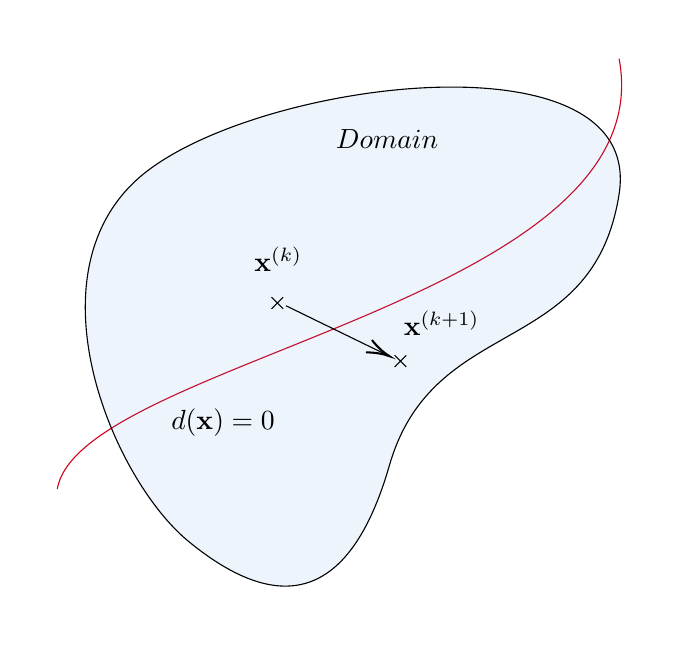
\begin{tikzpicture}[x=0.75pt,y=0.75pt,yscale=-1,xscale=1]
%uncomment if require: \path (0,310); %set diagram left start at 0, and has height of 310

%Curve Lines [id:da5390453303877039] 
\draw [color={rgb, 255:red, 208; green, 2; blue, 27 }  ,draw opacity=1 ]   (176.33,227.67) .. controls (187,165.67) and (469,137) .. (447,20.33) ;
%Shape: Polygon Curved [id:ds27867572621127656] 
\draw  [fill={rgb, 255:red, 74; green, 144; blue, 226 }  ,fill opacity=0.1 ] (215,78.33) .. controls (267.67,31) and (459.67,5.67) .. (447,85.67) .. controls (434.33,165.67) and (357.67,142.33) .. (336.33,216.33) .. controls (315,290.33) and (276.33,283) .. (239.67,253) .. controls (203,223) and (162.33,125.67) .. (215,78.33) -- cycle ;
\draw   (279.53,135.26) -- (285.14,140.86)(285.14,135.26) -- (279.53,140.86) ;
\draw   (338.86,163.26) -- (344.47,168.86)(344.47,163.26) -- (338.86,168.86) ;
%Straight Lines [id:da6123622539442625] 
\draw    (286.5,139.38) -- (334.54,162.79) ;
\draw [shift={(336.33,163.67)}, rotate = 205.99] [color={rgb, 255:red, 0; green, 0; blue, 0 }  ][line width=0.75]    (10.93,-3.29) .. controls (6.95,-1.4) and (3.31,-0.3) .. (0,0) .. controls (3.31,0.3) and (6.95,1.4) .. (10.93,3.29)   ;

% Text Node
\draw (270,109.73) node [anchor=north west][inner sep=0.75pt]    {$\mathbf{x}^{( k)}$};
% Text Node
\draw (342,140.4) node [anchor=north west][inner sep=0.75pt]    {$\mathbf{x}^{( k+1)}$};
% Text Node
\draw (230,187.73) node [anchor=north west][inner sep=0.75pt]    {$d(\mathbf{x}) =0$};
% Text Node
\draw (309.33,53.07) node [anchor=north west][inner sep=0.75pt]    {$Domain$};
\end{tikzpicture}
  \caption{迭代过程中碰撞的示意图:其中红色线表明$d = 0$,即发生了相交,也是内点法约束不能穿越的部分,蓝色部分表明可行域。}\label{fig:collision}
\end{figure}

如图\ref{fig:collision}所示,从$\mathbf x_n$到$\mathbf x_{n+1}$更新过程中,由于动力学解算的最小化问题中并不考虑碰撞,则可能穿越不可行区域,即发生了碰撞。如图\ref{fig:interpret-optimal}所示,假设 $\hat{\mathbf x} = \arg\min_{\mathbf{x}} I(\mathbf x) + \frac{1}{2}\|D_{z} \mathbf{x}-\mathbf{z} - \mathbf{u}_{z}\|_{W}^2$,从$\mathbf{x}$ 到$\hat{\mathbf{x}}$ 存在碰撞。

Lei 等人指出,对于IPC使用的障碍函数,其系数可以为$+\infty$。因此
\begin{equation}
  \mathbf{d}^{(k)}=\argmin{B(\mathbf d) = 0} \frac{\rho}{2} \| D_{d} \mathbf{x}^{(k)} - \mathbf{d} + \mathbf{u}_{d}\|_{2}^{2}
\end{equation}
其中的 $\mathbf d$ 还应满足无穿透条件,因此其最优解位置如图\ref{fig:interpret-optimal}所示。

\begin{figure}[hbt]
  \centering

\tikzset{every picture/.style={line width=0.75pt}} %set default line width to 0.75pt        

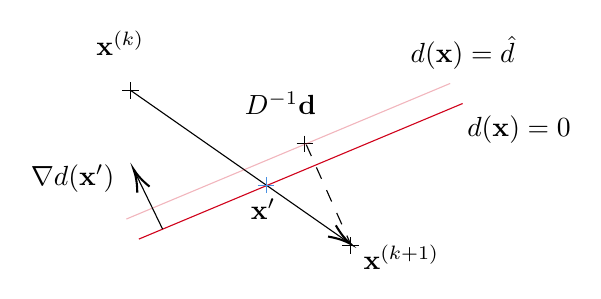
\begin{tikzpicture}[x=0.75pt,y=0.75pt,yscale=-1,xscale=1]
%uncomment if require: \path (0,300); %set diagram left start at 0, and has height of 300

\draw   (247.04,110.39) -- (254.96,110.39)(251,106.43) -- (251,114.36) ;
\draw   (353.04,185.06) -- (360.96,185.06)(357,181.1) -- (357,189.02) ;
%Straight Lines [id:da8691333295992784] 
\draw    (251,110.33) -- (355.36,183.19) ;
\draw [shift={(357,184.33)}, rotate = 214.92] [color={rgb, 255:red, 0; green, 0; blue, 0 }  ][line width=0.75]    (10.93,-3.29) .. controls (6.95,-1.4) and (3.31,-0.3) .. (0,0) .. controls (3.31,0.3) and (6.95,1.4) .. (10.93,3.29)   ;
%Straight Lines [id:da3846810796464156] 
\draw [color={rgb, 255:red, 208; green, 2; blue, 27 }  ,draw opacity=1 ]   (255,182) -- (411,116.67) ;
%Straight Lines [id:da34403059653345625] 
\draw  [dash pattern={on 4.5pt off 4.5pt}]  (335.67,136.5) -- (357,184.33) ;
\draw   (331.04,136.06) -- (338.96,136.06)(335,132.1) -- (335,140.02) ;
%Straight Lines [id:da7192719614800559] 
\draw [color={rgb, 255:red, 208; green, 2; blue, 27 }  ,draw opacity=0.29 ]   (249,172.33) -- (405,107) ;
%Straight Lines [id:da48171595095455455] 
\draw    (266.43,177.14) -- (253.3,150.09) ;
\draw [shift={(252.43,148.29)}, rotate = 64.12] [color={rgb, 255:red, 0; green, 0; blue, 0 }  ][line width=0.75]    (10.93,-3.29) .. controls (6.95,-1.4) and (3.31,-0.3) .. (0,0) .. controls (3.31,0.3) and (6.95,1.4) .. (10.93,3.29)   ;
\draw  [color={rgb, 255:red, 74; green, 144; blue, 226 }  ,draw opacity=1 ] (312.37,156.06) -- (320.3,156.06)(316.33,152.1) -- (316.33,160.02) ;

% Text Node
\draw (233.33,80.4) node [anchor=north west][inner sep=0.75pt]    {$\mathbf{x}^{( k)}$};
% Text Node
\draw (362,183.4) node [anchor=north west][inner sep=0.75pt]    {$\mathbf{x}^{( k+1)}$};
% Text Node
\draw (412,121.4) node [anchor=north west][inner sep=0.75pt]    {$d(\mathbf{x}) =0$};
% Text Node
\draw (304.83,109.73) node [anchor=north west][inner sep=0.75pt]    {$D^{-1}\mathbf{d}$};
% Text Node
\draw (384.67,83.07) node [anchor=north west][inner sep=0.75pt]    {$d(\mathbf{x}) =\hat{d}$};
% Text Node
\draw (201.71,144.83) node [anchor=north west][inner sep=0.75pt]    {$\nabla d(\mathbf{x} ')$};
% Text Node
\draw (307.67,161.07) node [anchor=north west][inner sep=0.75pt]    {$\mathbf{x} '$};


\end{tikzpicture}
\caption{计算$D^{-1}\mathbf d$:红色线为$d = 0$在$\mathbf x'$处的线性近似,$\nabla d(x')$为指向$\mathbf x^{(k)}$的法向。}\label{fig:interpret-optimal}
\end{figure}

为了加速其求解,将 $d(\mathbf x)$ 在碰撞处(即$d (\mathbf x')= 0$处)进行线性近似:
\begin{equation}
  d(\mathbf x) \approx (\nabla d(\mathbf x') )^T (\mathbf x  - \mathbf x')
\end{equation}
为使得$d = \hat d$,并利用距离函数$\|\nabla d\| \equiv 1$的性质,有
\begin{equation}
  D^{-1}\mathbf d = \mathbf x^{(k+1)} + (\hat d + (\nabla d(\mathbf x'))^T (\mathbf x' - \mathbf x^{(k+1)}))\nabla d(\mathbf x')
\end{equation}

另外,对于$k>1$时,第1步需要使用碰撞检测确定最大可行步长。令
\begin{equation}
  \tilde{\mathbf{x}}^{(k)}=\argmin{\mathbf{x}} I(\mathbf{x}) + \frac{1}{2} \| D_{z} \mathbf{x} - \mathbf{z}^{(k-1)} +\mathbf{u}_{z}^{(k-1)}\|_{W}^{2} +  \frac{1}{2} \| D_{d} \mathbf{x} - \mathbf{d}^{(k-1)} +\mathbf{u}_{d}^{(k-1)}\|_{2}^{2}
\end{equation}
以及 $t_{\min}=CCD(\mathbf{x}^{(k-1)}, \tilde {\mathbf{x}}^{(k)})$ 表示最近的碰撞时刻,则位置更新为:
\begin{equation}
  \mathbf x^{(k)} = t_{\min}\tilde{\mathbf x}^{(k)} + (1-t_{\min})\mathbf x^{(k - 1)}
\end{equation}
该算法利用每一步$\mathbf x^{(k)}\rightarrow \mathbf x^{(k+1)}$ 无碰撞来保证整个时间步内不发生穿透。而由于没有穿透发生,因此IPC在ADMM中的松弛变量$\mathbf u_d$ 恒为 0。

\section{算法描述}

总结以上内容,可得ADMM-IPC算法\ref{alg:ipc-fluid-final}。
\begin{algorithm}[H]
  \caption{ADMM-IPC}\label{alg:ipc-fluid-final}
  \begin{algorithmic}[1]
    \Require 系统各物体位置$\mathbf x^n$,速度$\mathbf v^n$,时间步长$h$
    \Ensure 积分结果 $\mathbf x^{n+1}, \mathbf v^{n+1}$
    \State $\mathbf x^{(1)} \leftarrow \mathbf [x^{n}, v^{n}], \mathbf u_z^{(0)} = \mathbf 0, k = 1$
    \While{not converged}
      \State $\mathbf z^{(k)} \leftarrow$ DynamicLocalStep()
      \State $\mathbf{u}_{z} ^{(k)} \leftarrow \mathbf{u}_{z}^{(k-1)} + (D_{z} \mathbf{x} ^{(k)}- \mathbf{z}^{(k)})$
      \State $\hat{\mathbf x}^{(k)} \leftarrow $DynamicGlobalStep()
      \State $\mathbf{d}^{(k)} \leftarrow \text{ContactLocalStep}(\mathbf{x}^{(k)}, \hat{\mathbf{x}}^{(k)})$
      \State $\hat{\mathbf{x}}^{(k)}\leftarrow \text{ContactGlobalStep}(\mathbf{d}^{(k)}, \hat{\mathbf{x}}^{(k)})$
      \State $t_I \leftarrow \text{CCD}(\mathbf x^{(k)}, \hat{\mathbf x}^{(k)})$
      \State $\mathbf{x}^{(k+1)} \leftarrow (1-t_{I}) \mathbf{x}^{(k)} +t_{I} \hat{\mathbf{x}}^{(k)}$
      \State $k \leftarrow k + 1$
    \EndWhile
  \end{algorithmic}
\end{algorithm}








\chapter{实现细节与结果分析}\label{chap:experiment}

\section{ADMM动力学解算}\label{sec:experiment-admm}

尽管前文已经给出了用于流固耦合的具体方法(算法\ref{alg:ipc-fluid-final}),但作为本设计的另一重要部分,本节将详细阐述基于ADMM方法实现的动力学求解算法,即DynamicLocalStep和DynamicGlobalStep的具体细节。

在\ref{sec:admm}中已经详细阐述了弹簧质点PD的算法(Local/Global),并分析了其与ADMM算法的联系。在本文具体的实现中,相较于PD算法,我们修改了$\rho = 1$。此时Local Step即为DynamicLocalStep,Global Step即为DynamicGlobalStep。

不同于原先PD的算法,我们在弹簧质点模型中使用了Consensus ADMM算法,类似于Jacobi迭代,是一个无矩阵的方法,非常利于并行计算实现。其修改了Global Step,相较于求解矩阵
\begin{equation}
  \mathbf A \mathbf x = \mathbf b
\end{equation}
其使用了单步的Jacobi迭代近似该方程的解:
\begin{equation}
 \left(\frac{m_i}{h^2} + \sum_{(i, j) \in \mathcal C} k_{ij}\right) \mathbf x^{(k+1)}_i = \frac{m_i}{h^2} \mathbf y_i + 
\sum_{(i, j)\in \mathcal C} k_{ij} (\mathbf x^{(k)}_j + \mathbf d) 
\end{equation}
该方法相较于原先的PD方法有较大的性能提升,如\ref{tab:ms}。
\begin{table}
  \centering
  \begin{tabular}{l|cc}
    模型尺寸& Consensus ADMM & PD\\
    \hline
    10$\times$10 & 1.4ms & 2.7ms \\
    100$\times$100 & 22ms & 75ms \\
    200$\times$200 & 80ms & 353ms
  \end{tabular}
  \caption{Consensus ADMM与PD对比:在不同场景下,Consensus ADMM相较于PD有2~5倍的性能提升。}\label{tab:mass-spring-benchmark}
\end{table}

\begin{figure}[hbt]
  \centering
  \includegraphics[width=0.8\linewidth]{img/mass-sp-result-norend.png}
  \caption{弹簧质点模型仿真结果}
\end{figure}

对于有限元法,DynamicLocalStep是对于每一个四面体$\mathbf D \mathbf x = [\mathbf x_2 - \mathbf x_{1},\mathbf x_3 - \mathbf x_{1}, \mathbf x_4 - \mathbf x_1]$,求解:
\begin{equation}
  \argmin{\mathbf Z} \frac{\rho}{2}\| \mathbf{Dx} - \mathbf{Z} \|_2^2 + u^{T} (\mathbf{Dx} - \mathbf{Z}) + \Phi(\mathbf Z)
\end{equation}
但考虑到\ref{eq:deformation-grad-compute},$\Phi$的计算依赖于形变梯度矩阵$\mathbf F = \mathbf Z\mathbf X_{rest}^{-1}$,为了减少计算 $\mathbf F$ 的开销,在这里存储形变梯度矩阵作为ADMM的松弛变量,而非直接为$\mathbf Z$,此时的ADMM的等式约束求解被转化为:
\begin{equation}
  \mathbf{Dx} - \mathbf{FX}_{rest}^{-1} = \mathbf 0
\end{equation}

其优点在于,在Local Step的迭代中,$\Phi(\mathbf F)$的实现是相对简单的,且不需要复杂的从$\mathbf X_{rest}$恢复对$\mathbf {Dx}$的操作。对于$\Phi$及其导数的实现,使用了基于Smith不变量的方法实现,而非传统的Cauchy不变量。尽管其只适用于一些简单模型,但其在实现上更为简单,计算更加高效,在图形学中较常用。

用于动力学求解的一个场景如图\ref{fig:hybrid-admm-result}所示。其性能能基本达到实时要求。(3\~10fps,其中有限元模型有400个节点,1384个四面体元, NeoHookean)

\begin{figure}[hbt]
  \centering
  \includegraphics[width=0.75\linewidth]{img/hybrid-admm.png}
  \caption{有限元法、弹簧质点模型统一场景仿真结果}\label{fig:hybrid-admm-result}
\end{figure}


\section{两阶段碰撞检测算法}\label{sec:collid-detect}

尽管ADMM-IPC算法已经完善,但通过分析解算占用的时间可以看到,CCD计算,即碰撞相关计算占据的时间相较其他步骤都高,因此在本章也将详细阐述本文实现的碰撞检测算法。通常而言,碰撞检测至少分为两阶段:
\begin{enumerate}
  \item 粗阶段:通常是建立空间数据结构(例如均匀网格、BVH、kd树及相关变体)并利用其进行快速的空间范围查找,初步确定可能碰撞的图元;
  \item 细阶段:对于给定的两个图元,确定其在时间步更新内是否存在相交;
\end{enumerate}

在粗阶段,不同于传统的BVH方法,粗阶段算法专为流体粒子这类小对象设计了特殊的多层均匀网格(Sparse Grid)。其最小单元为轴对齐包围盒(AABB),其拓扑结构类似于VDB:
\begin{figure}[hbt]
  \centering
  \subfigure[Sparse Grid]{
\tikzset{every picture/.style={line width=0.75pt}} %set default line width to 0.75pt
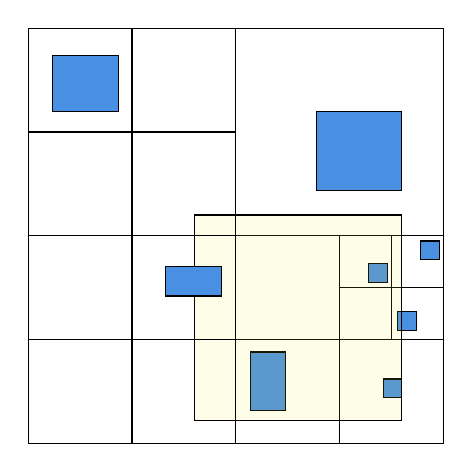
\begin{tikzpicture}[x=0.75pt,y=0.75pt,yscale=-1,xscale=1]
%uncomment if require: \path (0,300); %set diagram left start at 0, and has height of 300
%Shape: Grid [id:dp37542913168733505] 
\draw  [draw opacity=0] (211,35) -- (411,35) -- (411,235) -- (211,235) -- cycle ; \draw   (311,35) -- (311,235) ; \draw   (211,135) -- (411,135) ; \draw   (211,35) -- (411,35) -- (411,235) -- (211,235) -- cycle ;
%Shape: Grid [id:dp9750791482935114] 
\draw  [draw opacity=0] (311,135) -- (411,135) -- (411,235) -- (311,235) -- cycle ; \draw   (361,135) -- (361,235) ; \draw   (311,185) -- (411,185) ; \draw   (311,135) -- (411,135) -- (411,235) -- (311,235) -- cycle ;
%Shape: Grid [id:dp7892168057908815] 
\draw  [draw opacity=0] (361,135) -- (411,135) -- (411,185) -- (361,185) -- cycle ; \draw   (386,135) -- (386,185) ; \draw   (361,160) -- (411,160) ; \draw   (361,135) -- (411,135) -- (411,185) -- (361,185) -- cycle ;
%Shape: Rectangle [id:dp6060962911152178] 
\draw  [fill={rgb, 255:red, 74; green, 144; blue, 226 }  ,fill opacity=1 ] (318,191) -- (335,191) -- (335,219) -- (318,219) -- cycle ;
%Shape: Square [id:dp5321338766394932] 
\draw  [fill={rgb, 255:red, 74; green, 144; blue, 226 }  ,fill opacity=1 ] (400,137.5) -- (409,137.5) -- (409,146.5) -- (400,146.5) -- cycle ;
%Shape: Rectangle [id:dp15366556085797622] 
\draw  [fill={rgb, 255:red, 74; green, 144; blue, 226 }  ,fill opacity=1 ] (222.5,48.25) -- (254.5,48.25) -- (254.5,75.25) -- (222.5,75.25) -- cycle ;
%Shape: Square [id:dp12763621362581] 
\draw  [fill={rgb, 255:red, 74; green, 144; blue, 226 }  ,fill opacity=1 ] (375,148.5) -- (384,148.5) -- (384,157.5) -- (375,157.5) -- cycle ;
%Shape: Square [id:dp5679476241121324] 
\draw  [fill={rgb, 255:red, 74; green, 144; blue, 226 }  ,fill opacity=1 ] (389,171.5) -- (398,171.5) -- (398,180.5) -- (389,180.5) -- cycle ;
%Shape: Square [id:dp8942121948129986] 
\draw  [fill={rgb, 255:red, 74; green, 144; blue, 226 }  ,fill opacity=1 ] (382,204) -- (391,204) -- (391,213) -- (382,213) -- cycle ;
%Shape: Rectangle [id:dp04023637035985317] 
\draw  [fill={rgb, 255:red, 248; green, 231; blue, 28 }  ,fill opacity=0.1 ] (291,125) -- (391,125) -- (391,224) -- (291,224) -- cycle ;
%Shape: Grid [id:dp5558545847926403] 
\draw  [draw opacity=0] (211,135) -- (311,135) -- (311,235) -- (211,235) -- cycle ; \draw   (261,135) -- (261,235) ; \draw   (211,185) -- (311,185) ; \draw   (211,135) -- (311,135) -- (311,235) -- (211,235) -- cycle ;
%Shape: Grid [id:dp3022965469884248] 
\draw  [draw opacity=0] (211,35) -- (311,35) -- (311,135) -- (211,135) -- cycle ; \draw   (261,35) -- (261,135) ; \draw   (211,85) -- (311,85) ; \draw   (211,35) -- (311,35) -- (311,135) -- (211,135) -- cycle ;
%Shape: Rectangle [id:dp14826936005710334] 
\draw  [fill={rgb, 255:red, 74; green, 144; blue, 226 }  ,fill opacity=1 ] (350,75) -- (391,75) -- (391,113) -- (350,113) -- cycle ;
%Shape: Rectangle [id:dp86948007626014] 
\draw  [fill={rgb, 255:red, 74; green, 144; blue, 226 }  ,fill opacity=1 ] (277,150) -- (304,150) -- (304,164) -- (277,164) -- cycle ;
\end{tikzpicture}
}
\subfigure[OpenVDB实现]{\includegraphics[width=0.425\linewidth]{img/vdb.png}}
  \caption{空间数据结构的实现:左图蓝色表明空间中存在的AABB,黄色部分表明查找范围;右图为OpenVDB对于空间数据的存储方式。}
\end{figure}

构建空间数据结构的速度是碰撞检测的主要性能瓶颈,基于树的空间数据结构的一大问题是其相对难以进行并行。但Sparse Grid能够对已经排序好的一列AABB进行并行的构建,并能有效避免树的层数过高的问题。

Sparse Grid需要指定一个Cell的边长最大值$l$(通常为1),以及最大划分粒度 $k$。每一次进行空间划分都将空间划分为$2^3$份(xyz-轴各二等分),对于每一个边长为$l$的Cell,都至多进行$k$层划分。对于每一个AABB,其都尝试找到最适合的划分块插入。并行构建Sparse Grid的算法如下:

\begin{algorithm}
  \caption{Parallel Sparse Grid Build}\label{alg:ipc-fluid-final}
  \begin{algorithmic}[1]
    \Require 流体粒子包围盒 $\mathbf B$,Sparse Grid参数 $l, k$
    \Ensure Sparse Grid $G$
    \State 确定每一个流体粒子所在Sparse Grid中的位置,并按照边长为$l$的Cell编号排序
    \State 创建所需要的边长为$l$的Cell,并行地将所有排序后的粒子插入
  \end{algorithmic}
\end{algorithm}

在细阶段,本文沿用了基于三次方程的连续碰撞检测模型。记CCD起始点的流体、三角形顶点的位置分别为$\mathbf{f},\mathbf{x}_{1},\mathbf{x}_{2},\mathbf{x}_{3}$,以及更新位置$\mathbf{f}',\mathbf{x}'_{1},\mathbf{x}'_{2},\mathbf{x}'_{3}$其基于以下的方程求解:
\begin{equation}
  \exists t \in [0, 1]\quad \begin{cases}
\det \left[\mathbf x_{1,f} \mathbf x_{2,f}\mathbf x_{3,f}\right] = 0\\
\mathbf x_4 \in \triangle \mathbf x_1\mathbf x_2\mathbf x_3
\end{cases}
\end{equation}
其中$\mathbf x_{i,f} = t (\mathbf x_i ' -\mathbf f') + (1-t) (\mathbf x_i -\mathbf f)$

相对容易求解的是方程中的行列式部分,其是一个关于$t$的三次方程,本文实现的算法基于在区间$[0,1]$内三点进行牛顿迭代,确保不遗漏其在区间内的任一解。该算法能够进行快速求解,并在CCD-Benchmark中获得了其他求解器不拥有的性能优势,如表\ref{tab:ccd-benchmark}所示。

\begin{table}
\centering
\begin{tabular}{l|cccc}
   & IRF & TCCD & TI & 本文\\
  \hline
  t& 115.89 & 0.24 & 0.74 & 0.1 \\
  FP& 2 & 95638 & 2 & 2\\
  FN& 0 & 0 & 0 & 0
\end{tabular}
\caption{CCD-Benchmark结果:本文方法在求解速度、精确度、鲁棒性上都相比以往方法有极大的提升。}\label{tab:ccd-benchmark}
\end{table}

\subsection{ADMM-IPC结果}

基于以上内容,本文实现了ADMM-IPC算法,并在简单场景下进行了测试,下图展示了其流固耦合结果,场景设置为一斜放着的布料,与上方落下的水团进行耦合。

\begin{figure}
  \centering
  \includegraphics[width=0.9\linewidth]{img/well rendered-0001.png}
\end{figure}


\chapter{未来工作与展望}\label{chap:no-future}

\end{Main}
% References.
% TODO: References.
\begin{Acknowledgement}{}
这次的毕业论文设计总结是在我的指导老师xxx老师亲切关怀和悉心指导下完成的。从毕业设计选题到设计完成,x老师给予了我耐心指导与细心关怀,有了莫老师耐心指导与细心关怀我才不会在设计的过程中迷失方向,失去前进动力。x老师有严肃的科学态度,严谨的治学精神和精益求精的工作作风,这些都是我所需要学习的,感谢x老师给予了我这样一个学习机会,谢谢!

感谢与我并肩作战的舍友与同学们,感谢关心我支持我的朋友们,感谢学校领导、老师们,感谢你们给予我的帮助与关怀;感谢肇庆学院,特别感谢计算机科学与软件学院四年来为我提供的良好学习环境,谢谢!
\end{Acknowledgement}
% Thanks
\include{thanks}

\end{document}
